\begin{figure}[!htbp]
\centering
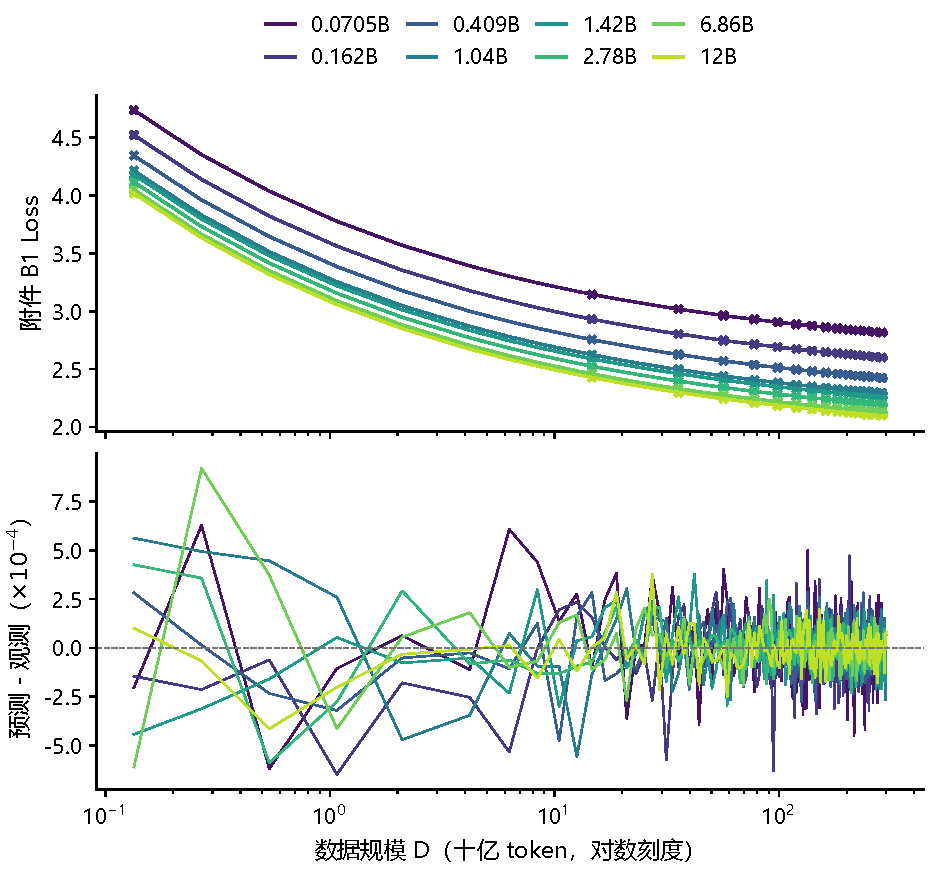
\includegraphics[width=15cm]{06_results/figures/round5/FIG-Q2-R5-001.pdf}
\caption{八条附件轨迹与幂律吻合；微小残差不证明外部真实性。}
\end{figure}
\begin{figure}[!htbp]
\centering
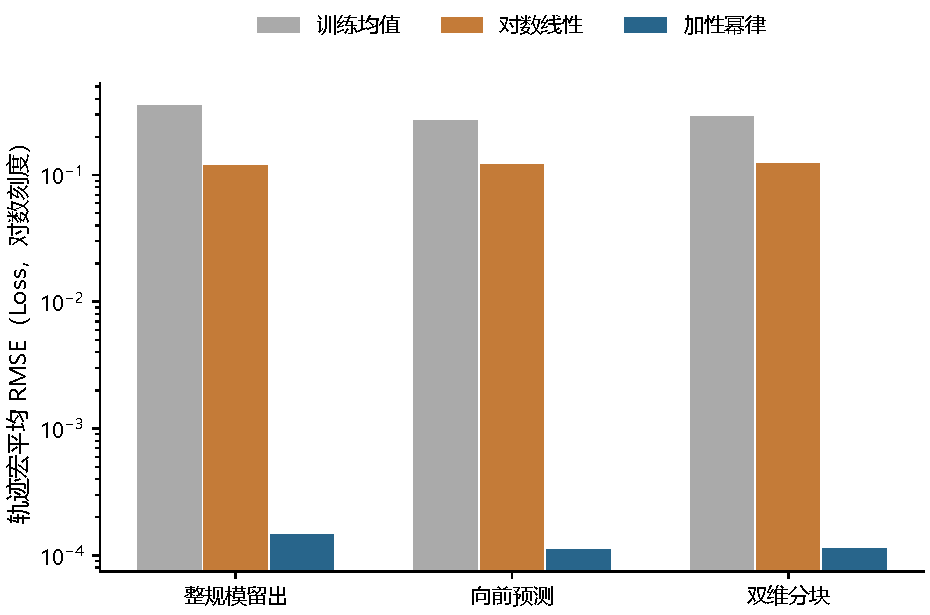
\includegraphics[width=15cm]{06_results/figures/round5/FIG-Q2-R5-002.pdf}
\caption{三类无随机拆行验证中，加性幂律优于两个透明对照。}
\end{figure}
\begin{figure}[!htbp]
\centering
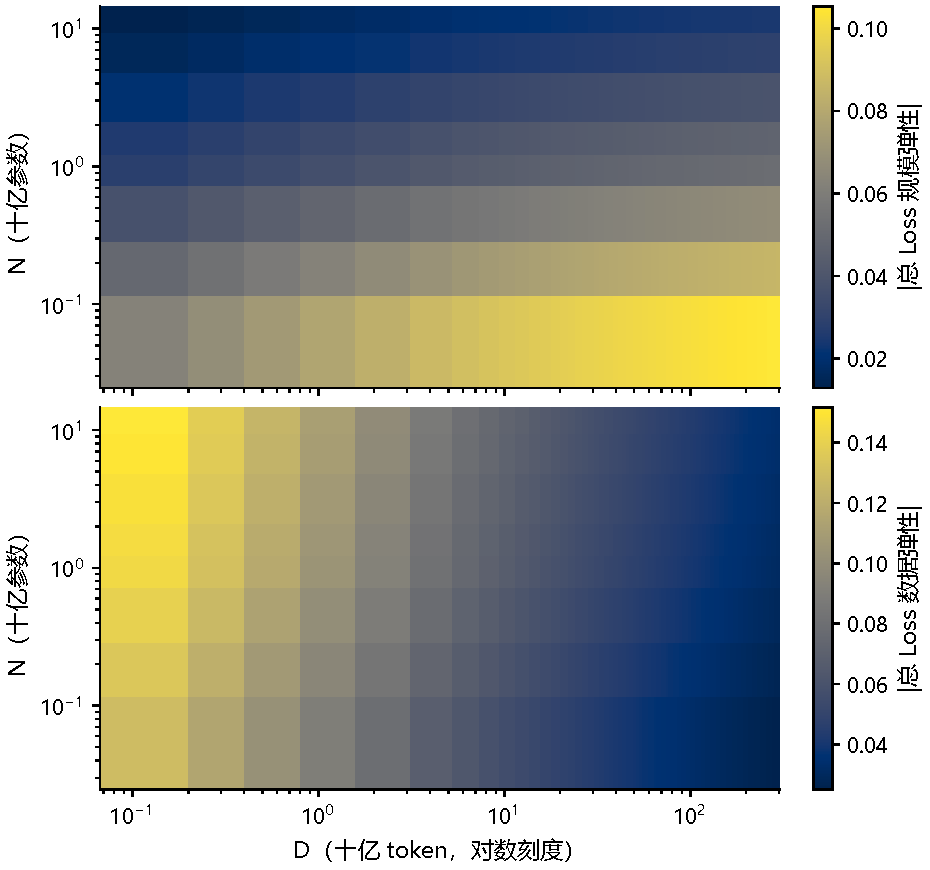
\includegraphics[width=15cm]{06_results/figures/round5/FIG-Q2-R5-003.pdf}
\caption{幂指数为常数，总Loss弹性随N-D状态变化。}
\end{figure}
\begin{figure}[!htbp]
\centering
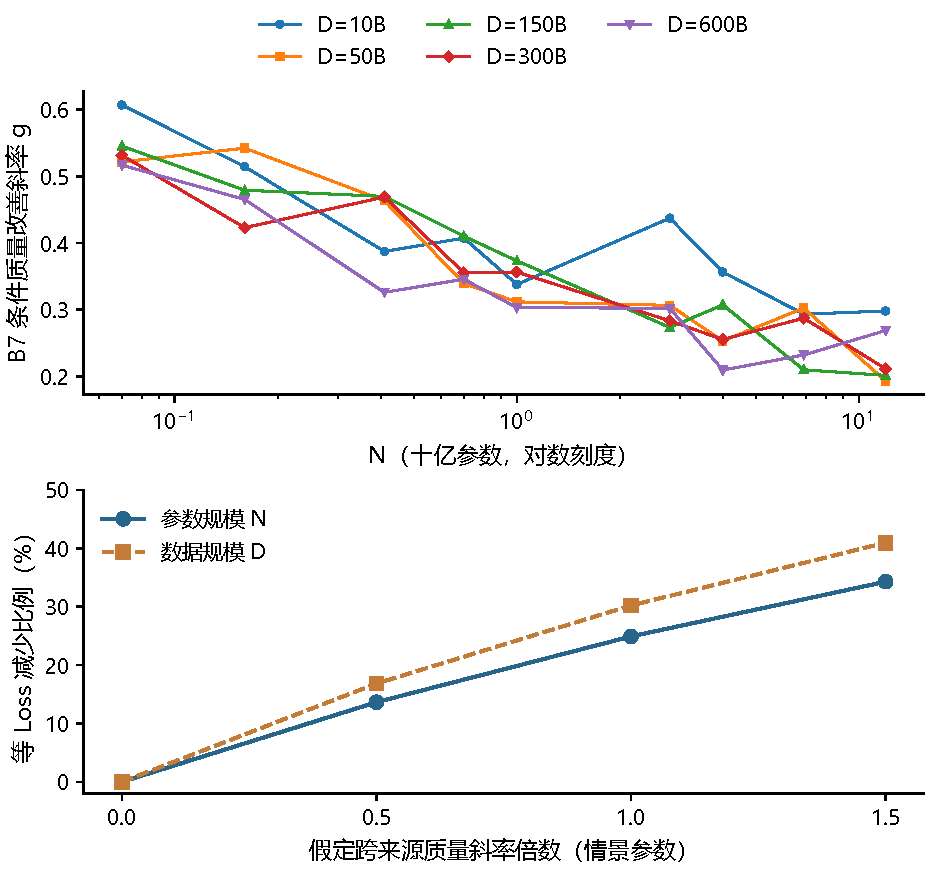
\includegraphics[width=15cm]{06_results/figures/round5/FIG-Q2-R5-004.pdf}
\caption{上图为半合成表内斜率；下图为假定Q从0.5增至0.6的替代情景，不能解释为真实收益。}
\end{figure}
